\documentclass{article}
\usepackage[preprint]{neurips}
\usepackage[utf8]{inputenc}
\usepackage[T1]{fontenc}
\usepackage{hyperref}
\usepackage{url}
\usepackage{booktabs}
\usepackage{amsfonts,amsmath}
\usepackage{nicefrac}
\usepackage{microtype}
\usepackage{graphicx}
\usepackage{xcolor}

\newcommand{\head}{\textsc{RimHead}}
\newcommand{\absrel}{\mathrm{AbsRel}}

\title{The Near-Field Rim: Diagnosing and Repairing Fisheye Depth in Frozen
3D Foundation Models Without Touching What Pose Needs}

\author{%
  Anonymous\\
  % camera-ready: fill in
}

\begin{document}

\maketitle

\begin{abstract}
We show that the fisheye-depth failure of frozen 3D foundation models is not
what it is assumed to be, and that fixing it correctly requires knowing what
the periphery is already doing. On Aria Digital Twin 110\textdegree{} fisheye,
we measure that (i) the depth error of a frozen model is a \emph{precise,
radially modulated range compression} --- per-region dispersion is only
2--10\% in log-depth while near-field content is placed up to $3.3\times$ too
far, worst at the rim; (ii) the rim is simultaneously the model's
\emph{alignment workhorse}: deleting all central content leaves its relative
pose essentially unchanged, while deleting the rim costs $3\times$ an
area-matched random control; and (iii) multi-frame context improves depth
almost exclusively in the center --- the rim powers cross-frame alignment but
receives none of the fusion gains. These measurements locate the practical
failure at the \emph{near-field rim}, which in egocentric video is precisely
where the wearer's hands live (80\%+ of hand pixels beyond
41\textdegree{}, median depth 0.26--0.94\,m). Because the compression is
many-to-one, output-indexed recalibration provably cannot invert it --- a
48-parameter lookup table transfers at the rim but corrupts the near center.
Instead, a 25k-parameter zero-initialized head reading the \emph{frozen}
backbone's own final patch tokens repairs the near-field rim by 51--75\% on
held-out frames, improves every other region, fits in minutes on a CPU, and
cannot move the pose path by construction. A single head trained on five
scenes transfers to a held-out sixth at or above within-scene gains
($-74.5\%$ to $-78.0\%$), and the recipe carries to a second backbone with
reduced effect. We release the full diagnosis protocol, including the
distance-controlled radial tables that separate ``the rim is hard'' from
``the rim looks at different content.''
\end{abstract}

\section{Introduction}
\label{sec:intro}

Egocentric devices ship fisheye cameras: Project Aria's RGB camera covers
$\sim$110\textdegree{} through a Kannala--Brandt lens. Frozen 3D foundation
models --- VGGT~\cite{vggt}, Depth Anything~3~\cite{da3},
$\pi^3$~\cite{pi3} --- are trained overwhelmingly on perspective imagery, and
their depth degrades toward the fisheye rim. A growing family of
parameter-efficient adapters responds by modifying the backbone's input or
computation: positional-encoding residuals~\cite{raytun3r}, calibration
tokens~\cite{fisheye3r,caltokens}, low-rank updates inside attention
blocks~\cite{depthfisheye}. All of them report whole-image means, and none
asks two questions this paper treats as primary: \emph{what exactly is broken
at the rim}, and \emph{what is the rim already doing that a repair must not
disturb?}

We answer both by measurement on Aria Digital Twin (ADT)~\cite{adt}, then let
the measurements dictate a deliberately minimal repair. Our contributions:

\begin{itemize}
  \item \textbf{A diagnosis} (\S\ref{sec:broken}): with a ground-truth-depth
  control that separates field position from scene content, and an
  alignment-free bias/dispersion decomposition, the radial failure is a
  \emph{precise miscalibration} --- a depth-range compression around the frame
  level, radially modulated --- not noise. Dispersion is 2--10\% everywhere;
  bias reaches $3.3\times$ at the near rim.
  \item \textbf{An asymmetry} (\S\ref{sec:periphery}): count-matched
  correspondence experiments and masking with area-matched random controls
  show the rim's pose value is angular \emph{span under real noise} (not
  per-point quality), that a frozen model's pose relies on the rim (center
  deletion is free; rim deletion costs $2.6\times$), and --- combined with a
  six-sequence multi-frame study --- that \emph{context buys the center, not
  the field}: the rim gives alignment and does not receive depth.
  \item \textbf{A minimal safe repair} (\S\ref{sec:method}): the compression
  is many-to-one in true depth, so any correction indexed by the model's
  output alone provably conflates populations --- measured as near-center
  collateral of a 48-parameter table. A zero-initialized $\sim$25k-parameter
  MLP on the frozen backbone's final patch tokens disambiguates: near-field
  rim $\absrel$ falls 51--75\% on held-out frames across six sequences with
  every other zone improving, pose untouched by construction. One head
  trained on five scenes transfers to the sixth at $-74.5$ to $-78.0\%$.
  \item \textbf{Negative results with mechanisms}: per-patch content
  undistortion is a non-mechanism at this lens class (within-patch distortion
  $\le 0.21$\,px --- quantifying why an ablation row in \cite{raytun3r} is
  small); hands, despite living exactly in the failure zone, act as plain
  occlusion rather than signal corruption.
\end{itemize}

Throughout, every comparison carries three axes --- center depth, rim depth,
and pose stability --- because our own measurements show the single
whole-image mean hides both the failure and the collateral damage of naive
fixes.

\section{Related work}
\label{sec:related}

\paragraph{Adapting geometry models to fisheye.}
RayTun3R~\cite{raytun3r} learns polar-binned residuals on positional
encodings of a frozen backbone per sequence; Fisheye3R~\cite{fisheye3r} and
calibration tokens~\cite{caltokens} insert learned tokens;
DepthFisheye~\cite{depthfisheye} applies LoRA inside attention blocks;
OmniVGGT~\cite{omnivggt} retrains a camera-conditioned side branch. All
modify the computation that \emph{both} depth and pose read from. Our repair
is readout-only: the backbone's forward pass is bit-identical, which is what
makes the pose-safety claim structural rather than empirical.
DrivingDepth~\cite{drivingdepth} corrects output scale pixel-wise but
requires sparse depth prompts at test time; our head needs only the model's
own tokens.

\paragraph{Diagnosing wide-FoV failure.}
UniK3D~\cite{unik3d} names the wide-FoV \emph{contraction} its angular loss
exists to prevent; our alignment-free maps measure exactly this contraction
on a frozen model, in 2D (angle $\times$ depth), and show it is nearly
noise-free. Depth-Any-Camera~\cite{dac} supplies the equirectangular
evaluation lineage. The distance confound in radial error curves --- the rim
of an indoor lens looks at nearer furniture --- is, to our knowledge, first
controlled explicitly here and in the companion benchmark tables we build on.

\paragraph{Wide field of view and pose.}
That outer-FoV features stabilize SLAM is folklore with classical
evidence~\cite{lfvislam}. We give it a foundation-model-era form and a
mechanism: at fixed correspondence count the value of span is robustness to
real feature noise (a $20\times$ larger effect than ideal-geometry
conditioning), and frozen feed-forward models already exploit it.

\section{What the periphery is for}
\label{sec:periphery}

\begin{figure}[t]
  \centering
  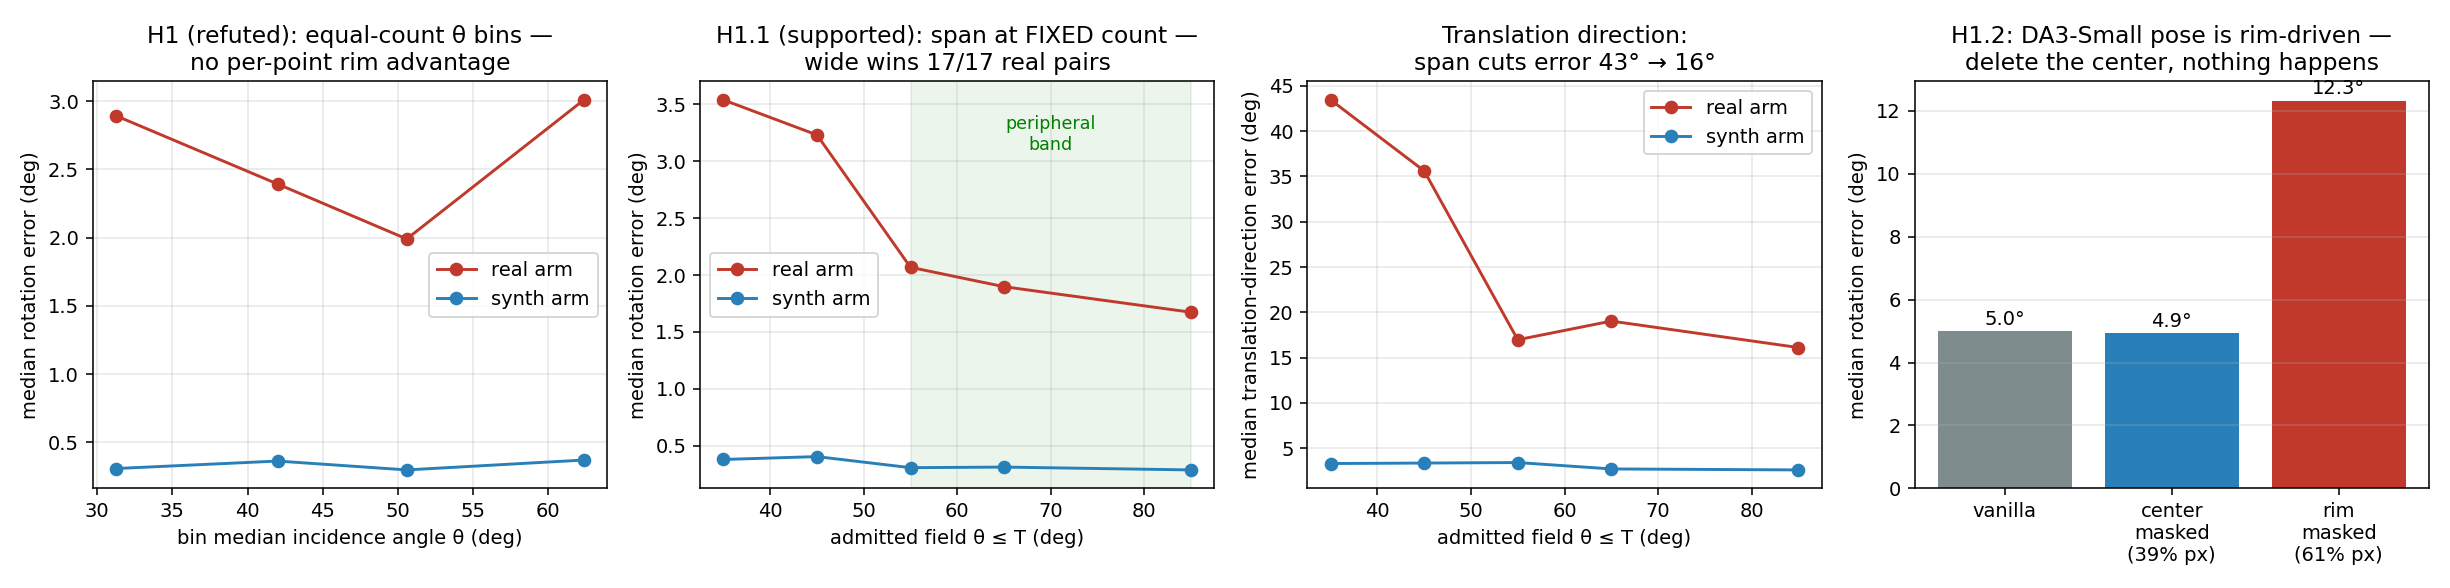
\includegraphics[width=\linewidth]{figures/h1_family.png}
  \caption{\textbf{The rim's pose value is span, not per-point quality; the
  frozen model already uses it.} Left to right: (a) equal-count incidence
  bins show no per-point rim advantage, and a synthetic control (same pixels,
  ideal noise) is flat; (b) at fixed count, admitting a wider field improves
  rotation on 17/17 real pairs while the ideal-noise control barely moves ---
  the mechanism is robustness to real matching noise; (c) the same for
  translation direction (43\textdegree$\to$16\textdegree); (d) masking DA3's
  input: deleting the entire center changes nothing, deleting the rim more
  than doubles error. ScanNet++ 170\textdegree{} scene; Aria replication in
  \S\ref{sec:periphery}. }
  \label{fig:h1}
\end{figure}

We first establish, classically and on the frozen model, what the rim
contributes to cross-frame alignment (Figure~\ref{fig:h1}).

\paragraph{No per-point rim advantage.} Splitting SIFT correspondences into
equal-count incidence-angle quartiles and estimating relative rotation per
bin (MAGSAC++ on bearings, with a lens-fair angular inlier rule), the rim bin
is no better than the center bin --- paired differences are a coin flip, and a
synthetic-bearing control with identical geometry and 1\,px noise is flat
across bins. Designs premised on ``rim points are individually more
informative'' have no basis.

\paragraph{Span under real noise.} Holding correspondence count fixed and
widening the admitted disk $\theta\le T$: real-data rotation error falls
monotonically (median $-2.15$\textdegree{} from $T{=}35$\textdegree{} to
$85$\textdegree{}, wide better on 17/17 pairs) and translation-direction
error falls from 43\textdegree{} to 16\textdegree{}. The identical protocol
on ideal-noise synthetic bearings shows $\sim$5\% of that effect. The
periphery's value is \emph{coverage that decorrelates real errors}. On Aria
(110\textdegree), the same curve replicates
(10.1\textdegree$\to$1.6\textdegree{} from $\theta\le25$\textdegree{} to
$\le$45\textdegree) and saturates by $\sim$45\textdegree.

\paragraph{The frozen model runs its pose on the rim.} Feeding DA3-Small
masked inputs: deleting all central content ($\theta\le45$\textdegree, 39\%
of pixels) leaves median rotation error unchanged (4.93\textdegree{} vs
5.00\textdegree); deleting the rim (61\%) costs 12.32\textdegree{} ---
$3\times$ the cost of an area-matched random patch mask (7.41\textdegree).
On Aria the ordering persists (rim-masked 38.5\textdegree{} $\gg$
area-matched random 25.3\textdegree{} $>$ center-masked 20.0\textdegree{}
$>$ vanilla 14.8\textdegree), with the softer center dependence expected of
a narrower cone. \emph{Any rim repair must therefore leave the features the
pose path reads intact} --- the design constraint the rest of the paper obeys.

Ground truth on ADT uses the factory device-to-camera calibration; where it
was initially unavailable we recovered the conjugation by rotation-only
hand-eye calibration from classical poses, gated at $<1.5$\textdegree{}
residual (achieved 0.77--0.96\textdegree), and later confirmed against the
factory value (2.33\textdegree{} apart).

\section{What is actually broken}
\label{sec:broken}

\begin{figure}[t]
  \centering
  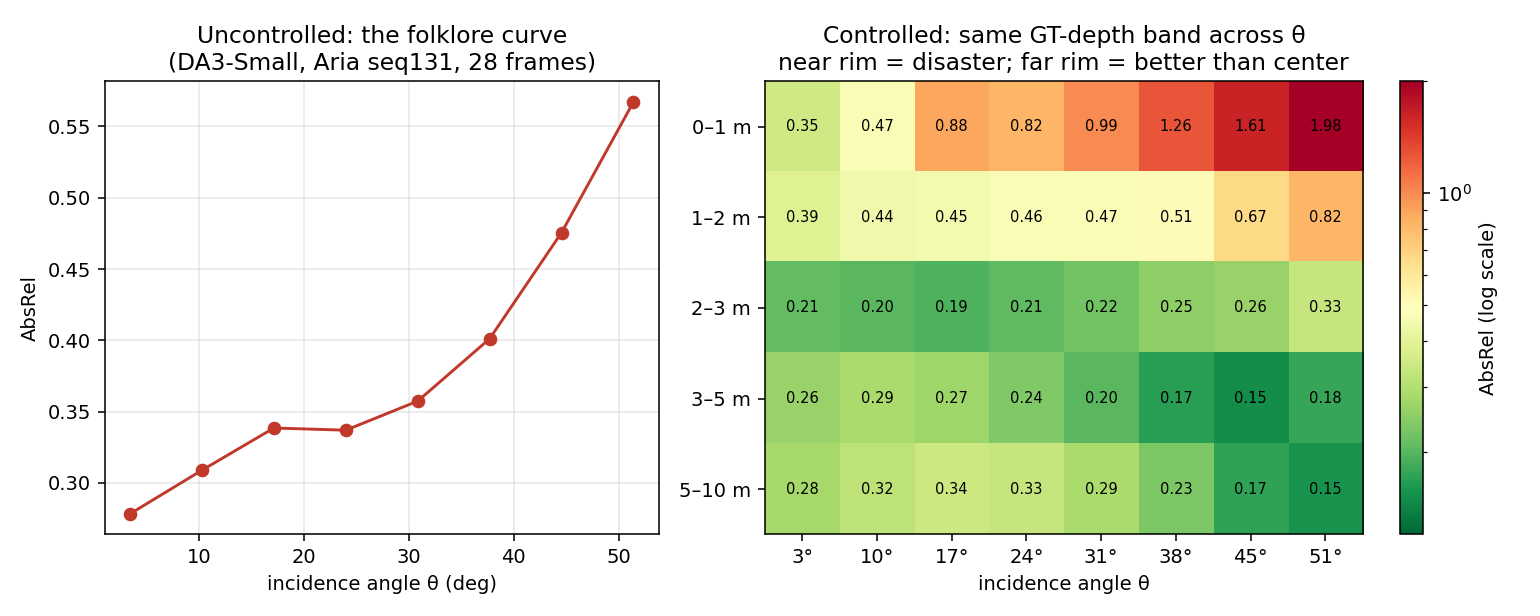
\includegraphics[width=\linewidth]{figures/depth_baseline_h20.png}
  \caption{\textbf{The radial failure is radial}$\times$\textbf{depth, and it
  is calibration, not noise.} Left: the uncontrolled radial curve. Right: the
  same prediction scored inside fixed ground-truth depth bands. Near bands
  (0--3\,m) degrade steeply toward the rim; far bands \emph{invert}. An
  alignment-free decomposition attributes nearly all of it to bias
  (range compression), with 2--10\% dispersion everywhere.}
  \label{fig:diag}
\end{figure}

Radial error curves confound field position with scene content: the rim of
an indoor fisheye looks at nearer surfaces. Scoring a frozen DA3-Small
prediction inside fixed GT-depth bands (Figure~\ref{fig:diag}) shows the
folklore curve (spread $2.04\times$) decomposes into a steep genuine
degradation at 0--3\,m (row spread up to $5.7\times$) and an
\emph{inversion} at 3--10\,m: far content is predicted \emph{better} at the
rim than at the center. A companion six-sequence, five-model study confirms
the raw-fisheye rim penalty survives the depth control across models
(controlled rim/center ratios 1.25--1.81$\times$) while rectified input's
penalty collapses to $\approx$1 --- and that adding 3/5/10 frames of context
improves overall depth while the rim/center ratio stays flat or worsens:
\textbf{context buys the center, not the field}.

Removing all alignment (per-cell median log-residual relative to the frame's
own level, and MAD around the cell median) shows why: dispersion is only
0.02--0.10 in log-depth \emph{everywhere, including the near rim}, while
bias is large and structured --- 0--1\,m content placed $e^{0.53}$ to
$e^{1.20}$ ($1.7$--$3.3\times$) too far, worsening with angle; 5--10\,m
content $1.4$--$1.8\times$ too near. The model \emph{sees} the near rim
fine; it mis-scales it, systematically and precisely. This is the frozen-model
analogue of the contraction UniK3D trains against~\cite{unik3d}.

Finally, the failure zone is not academic. On ADT skeleton sequences, hand
and body pixels are 0.8--4\% of the imaged cone, 80\%+ of them beyond
$\theta{=}41$\textdegree, at median depth 0.26--0.94\,m (verified against
both ADT depth-render variants: the with-skeleton render contains the person;
100\% of dynamic pixels differ from the person-free render by $>5$\,cm).
\textbf{The near-field rim is the hand zone.} Masking experiments show hands
nonetheless act as plain occlusion for pose --- ground-truth-mask deletion
beats an area-matched random mask by only 0.35--1.0\textdegree{} on
10--25\textdegree{} baselines --- so the repair needs hygiene (exclude dynamic
cells from fitting), not a dynamics-specific mechanism.

\section{A minimal safe repair}
\label{sec:method}

\begin{figure}[t]
  \centering
  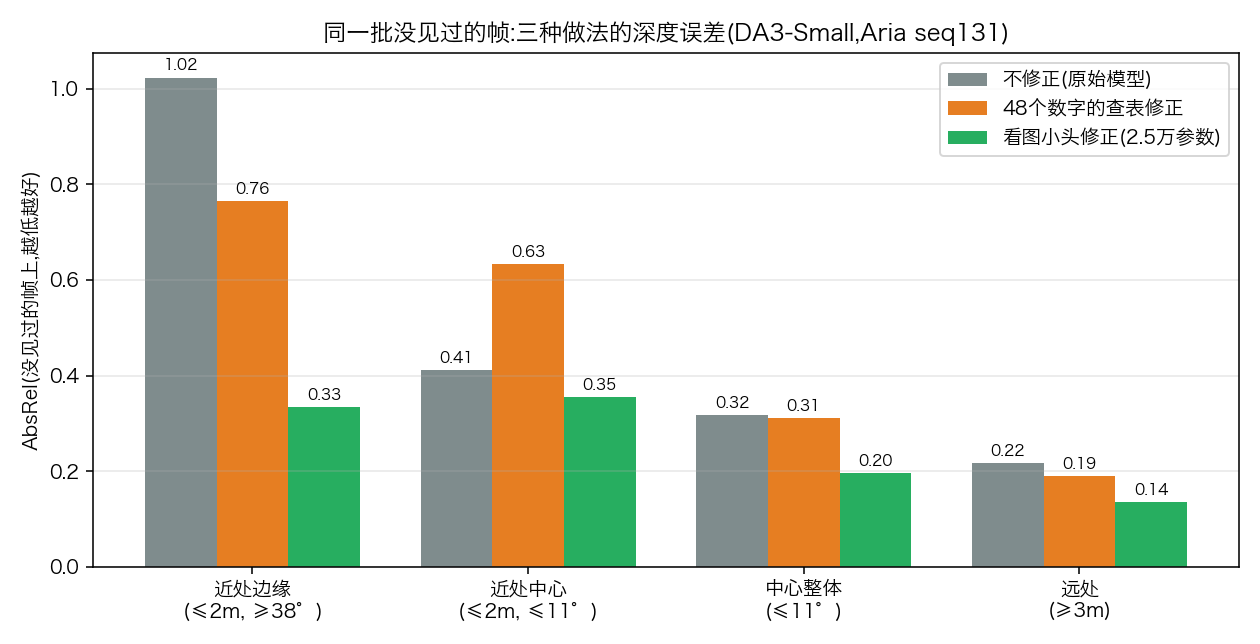
\includegraphics[width=.72\linewidth]{figures/feature_head_h22.png}
  \caption{\textbf{Output-indexed recalibration cannot invert a compression;
  frozen features can.} Held-out frames, seq131. The 48-parameter
  $(\theta\times\hat d\,)$ table (orange) transfers at the near rim but
  corrupts the near center --- the compression maps different true depths to
  the same prediction, so a correction indexed by the output pushes the
  majority's fix onto minorities. The 25k-parameter head on frozen tokens
  (green) beats it everywhere and removes the collateral.}
  \label{fig:head}
\end{figure}

\paragraph{Rung 1: the strongest trivial baseline.} If the failure is a fixed
miscalibration, a lookup should fix it: $d' = d\cdot\exp c[i,j]$ with
$8\times6$ bins over (incidence angle, \emph{predicted} log-depth), fitted as
per-cell median residuals on training frames. It transfers at the near rim
($-18$ to $-25\%$ held-out) --- and consistently corrupts the near center,
\emph{including with the evaluation affine frozen}. The mechanism is
structural: compression is many-to-one, so populations with different true
depths share a predicted-depth bin, and no function of the output can
separate them. Input evidence is necessary, not stylistic.

\paragraph{Rung 2: the head.} Per patch, we concatenate the frozen backbone's
final-layer token (LayerNormed), $\sin\theta,\cos\theta$ at the patch center,
and the patch's predicted log-depth; a two-layer MLP
($C{+}3\to64\to1$, $\sim$25k parameters, final layer zero-initialized)
predicts a per-patch multiplicative log-depth correction, bilinearly
upsampled. Training minimizes $L_1$ on frame-level-free log residuals ---
14 frames, $\sim$300 full-batch epochs, \emph{minutes on a laptop CPU}.
The backbone is untouched: its forward pass, and therefore its pose output,
is bit-identical --- pose safety by construction, not by measurement.
Dynamic-labelled cells are excluded from the loss.

\section{Experiments}
\label{sec:experiments}

\begin{figure}[t]
  \centering
  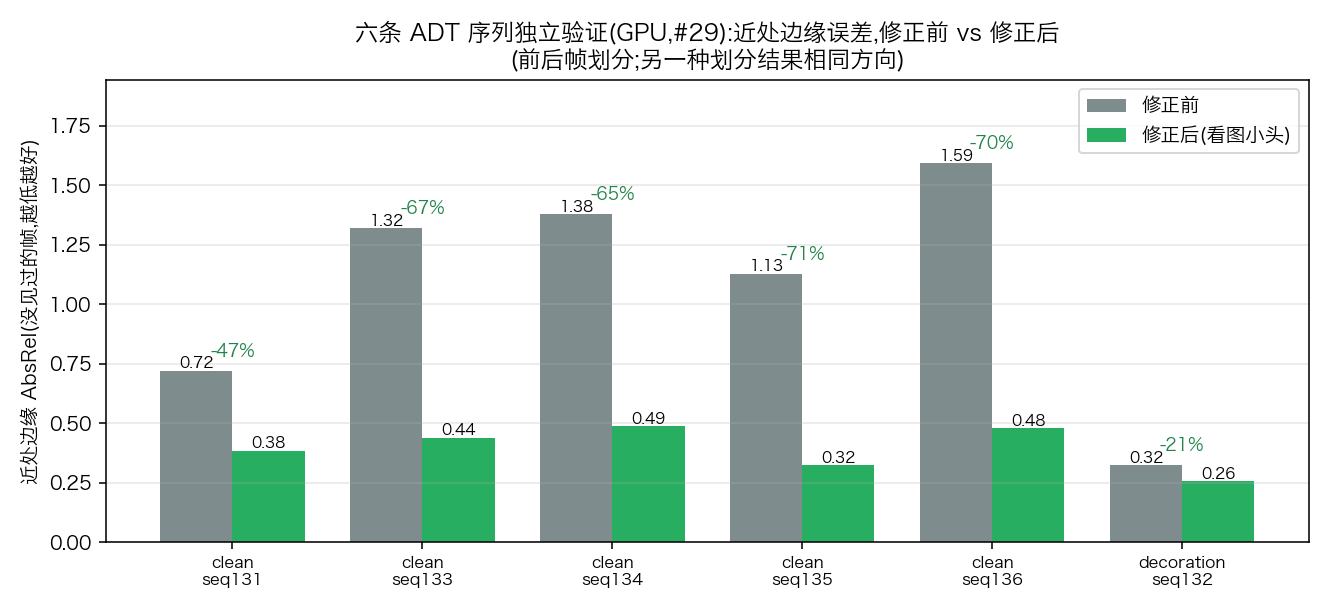
\includegraphics[width=\linewidth]{figures/sixseq_h22.png}
  \caption{\textbf{Six-sequence validation.} Near-field-rim $\absrel$ on
  held-out frames, before vs.\ after the head, per ADT sequence
  (temporal-halves split; the interleaved split agrees). Improvements range
  $-21\%$ to $-75\%$; near-center worst case $+5.8\%$ (noise-order).}
  \label{fig:sixseq}
\end{figure}

\paragraph{Protocol.} Range-domain $\absrel$ under one scale-shift affine per
frame frozen before any binning; joint (incidence $\times$ GT-depth) tables
reported in full --- zone aggregates provably hid the table baseline's
collateral. Zones: near rim ($\le$2\,m, $\ge$38\textdegree), near center
($\le$2\,m, $\le$11\textdegree), center, far.

\paragraph{Within-scene, six sequences.} (Figure~\ref{fig:sixseq}.) Near-rim
$\absrel$ improves on every sequence and both splits ($-21\%$ to $-75\%$;
5/6 sequences clear $-30\%$ on both splits); the near center is never
damaged beyond $+5.8\%$; center and far zones improve throughout. The
48-parameter table, by contrast, damages the near center wherever it helps
the rim.

\paragraph{Cross-scene: one head, not six.} Leave-one-scene-out over the six
sequences: on all five clean-apartment folds the cross-scene head matches or
exceeds the within-scene gain ($-74.5\%$ to $-78.0\%$ near-rim). The
visually distinct decoration sequence still clears the pre-registered bar
($-18.7\%$, $\ge$ half of within-scene) but shows real center collateral
($+27.8\%$) --- the honest boundary of a single head is visual genre, not
scene identity.

\paragraph{Backbone transfer.} The identical recipe on VGGT-$\Omega$ (the
backbone with the largest distance-controlled rim penalty, $1.81\times$)
improves the near rim on all 12 sequence$\times$split runs ($-19.3\%$ to
$-40.6\%$) but neither reaches DA3-Small's effect size nor its cleanliness
(near-center collateral up to $+49.8\%$ on temporal-halves splits). Its
final-layer tokens carry less of the disambiguating signal --- consistent with
an architecture whose single dense head couples depth to a self-estimated
field of view; probing earlier blocks is future work. The three-axis
protocol is what exposes this: whole-image means would call both backbones a
success.

\paragraph{Why not patch-level distortion adaptivity.} Correct per-patch
local undistortion (Jacobian-matched, identity at each patch center) changes
no cell of the joint table beyond the third decimal --- because on a
110\textdegree{} Kannala--Brandt lens at 14\,px patches, the within-patch
deviation of the true map from its linearization is $\le0.21$\,px even at
the rim. The distortion lives \emph{between} patches, in token geometry ---
where PE-residual methods~\cite{raytun3r} operate and where our diagnosis
already acts. This quantifies why that family's patch-resampling ablations
are small, and closes patch-content adaptivity for this lens class.

\section{Limitations}
\label{sec:limitations}

One lens class (110\textdegree{} KB4) and one capture domain (indoor ADT);
the within-patch-linearity argument must be re-measured for wider lenses.
Metric scale is freed per frame by the evaluation protocol; the head corrects
relative structure, not global scale. Cross-scene transfer is demonstrated
within visual genre and breaks partially across it. On VGGT-$\Omega$ the
repair is real but weaker and with center collateral --- readout-only repair
is pose-safe by construction, but \emph{center-depth} safety is empirical
and backbone-dependent. The classical span analysis on Aria rests on 11
pairs beyond 45\textdegree{} and cannot yet certify the outermost ring's
pose value. Multi-frame routing --- delivering the fusion gains the center
currently monopolizes to the rim --- is the natural next rung and untested.

\section{Conclusion}

Measured carefully, the fisheye failure of frozen 3D foundation models is a
precise, radially modulated range compression sitting exactly where
egocentric content matters most (the near-field rim, where hands live) and
exactly where the models' own cross-frame alignment comes from. That pairing
dictates the repair: input-conditioned, readout-only, zero-initialized ---
and it turns out 25k parameters and minutes of CPU fitting suffice to remove
half to three quarters of the near-rim error without touching what pose
needs. The broader lesson is methodological: adapters for wide-FoV geometry
should be judged on (center, rim, pose) jointly, with distance-controlled
tables --- the whole-image mean has been hiding both the disease and the side
effects of the cures.

\begin{thebibliography}{20}
% NOTE: entries below are assembled from the repository's verified survey
% (docs/research/fisheye-wide-fov-adaptation.md, each checked against its
% arXiv abstract page) — a programmatic BibTeX fetch pass is still required
% before submission; see paper/CITATIONS-TODO.md.
\bibitem{vggt} Wang et al. \emph{VGGT: Visual Geometry Grounded Transformer.} arXiv:2503.11651.
\bibitem{da3} ByteDance Seed. \emph{Depth Anything 3.} arXiv:2511.10647.
\bibitem{pi3} Wang et al. \emph{$\pi^3$: Permutation-Equivariant Visual Geometry Learning.} arXiv:2507.13347.
\bibitem{raytun3r} Sinitsyn, Araslanov, Cremers. \emph{RayTun3R: Online Camera Adaptation in 3D Foundation Models.} arXiv:2607.02711.
\bibitem{fisheye3r} Duan et al. \emph{Fisheye3R: Adapting Unified 3D Feed-Forward Foundation Models to Fisheye Lenses.} arXiv:2603.28896.
\bibitem{caltokens} \emph{Extending Foundational Monocular Depth Estimators to Fisheye Cameras with Calibration Tokens.} arXiv:2508.04928.
\bibitem{depthfisheye} \emph{DepthFisheye: Efficient Fine-Tuning of Depth Estimation Models for Fisheye.} ICCVM 2025. % [PLACEHOLDER — verify venue/authors]
\bibitem{omnivggt} \emph{OmniVGGT: Omni-Modality Driven Visual Geometry Grounded Transformer.} arXiv:2511.10560.
\bibitem{drivingdepth} \emph{DrivingDepth: Sparse-Prompted Pixel-wise Scale Correction for Driving Depth Estimation.} arXiv:2606.31488. % [PLACEHOLDER — verify]
\bibitem{unik3d} Piccinelli et al. \emph{UniK3D: Universal Camera Monocular 3D Estimation.} arXiv:2503.16591.
\bibitem{dac} Guo et al. \emph{Depth Any Camera: Zero-Shot Metric Depth Estimation from Any Camera.} arXiv:2501.02464.
\bibitem{lfvislam} Wang et al. \emph{LF-VISLAM: A SLAM Framework for Large Field-of-View Cameras.} arXiv:2209.05167.
\bibitem{adt} Pan et al. \emph{Aria Digital Twin: A New Benchmark Dataset for Egocentric 3D Machine Perception.} % [PLACEHOLDER — fetch canonical]
\end{thebibliography}

\end{document}
